\documentclass[12pt]{article}
\usepackage{graphicx}
\usepackage[utf8]{inputenc}
\usepackage[nottoc]{tocbibind}
\usepackage{graphicx}
\usepackage{wrapfig}
\usepackage{url}
\usepackage{listings}

%opening
\title{Linear Algebra in Autonomous Mobile Robots}
\author{Ethan Puerto, Stephen Chandler, Rhett Fitchett}

\begin{document}

\maketitle
\tableofcontents
\newpage
\begin{abstract}
In a world as modernized as ours, we tend to never take time to realize the inner workings of the various technologies around us. Everything from cell phones to microwaves contain bits of code or even devices that are foreign to every engineer and computer scientist other than those who created it. Linear algebra is everywhere especially in the world of modern robotics, autonomous localization, navigation, and route calculation. In this paper we will discuss the behind the scenes of what has been mentioned to help shine a light on the necessity of linear algebra in our modernizing world.
\end{abstract}

\newpage
\section{Introduction}
\quad Nearly every American has a cell phone in their pocket at all times. It has quickly become our most important lifeline. It allows us to communicate, learn, and even navigate. Every aspect of that device involves some form of linear algebra, and so do many aspects from different technologies used every day. For this paper, we are going to take the red pill and see how far the rabbit hole of linear algebra goes. One of the most interesting and rapidly growing technologies in the news is the research and tests being done in the field of Autonomous Robotics. Because cell phones are found in almost everyone’s pocket, many have been guilty of the epidemic of “texting and driving”, which has been estimated to cause about 1 in 4 motor vehicle accidents \cite{statistics}. \newline


With the increasing number of vehicle related deaths on the world’s roadways, interest and research into the “self-driving” or autonomous vehicle has grown rapidly. While the first experiments into autonomous vehicles started in the 1950s and 1960s, they were not truly autonomous as they usually relied on some sort of electrical guidance system that was implemented into the roadway. A great example of this is General Motors’ Firebird II, that would be able to self-steer through a guidance system embedded in the roadway. 
\newline

True autonomous vehicles did not begin to seem plausible until the innovations of the past decade or so. With the improvements in sensors, navigation systems, and computing power, companies like Google and Tesla are well underway into producing a fully autonomous vehicle that is readily available to the consumer. The most current implementations of autonomous cars rely on several systems in order to work, but we are going to focus on the image sensors and image recognition, GPS, and software that allows autonomous cars to detect obstacles in the roadway, determine its location on the globe, and determine the best route to get from point A to point B.\cite{GoogleCar}


\newpage
\section{GPS Navigation}
\quad Nearly every American has a cell phone in their pocket at all times. It has quickly become our most important lifeline. It allows us to communicate, learn, and even navigate. Every aspect of that device involves some form of linear algebra, but here, we are going to focus on the navigation and image recognition aspects because they directly apply to Autonomous Mobile Robotics.\newline

Navigation in our world has been simplified dramatically since the times of Columbus or Magellan. Since the use of hyperbolic navigation in World Wars I and II, finding our way around the globe has gotten significantly easier. To summarize, “Hyperbolic navigation is achieved when synchronized signals, having a known velocity of propagation, are transmitted from at least three known points, and when the relative times of arrival of these signals are measured and interpreted by a navigator." \cite{hyperNavigation}. This form of localization was widely known as LORAN, or in some variations LORAN-C. In short, by calculating the vectors to three known points in space LORAN is able to quite literally triangulate a given location. \newline

Over the years LORAN gave way to the arrival of the Global Positioning System, or GPS for short. GPS operates by the same mathematical premise, but rather than using radio towers on Earth, GPS uses orbiting satellites to triangulate position. The accuracy and power usage difference is what really sets the two systems apart. LORAN was used almost exclusively by marine vessels, where the large power consumption and an accuracy of roughly 5-10 miles was acceptable. For high accuracy uses however, it falls short of what GPS can provide. \newline

The use of GPS in autonomous robotics is essential for navigation. It allows for a standardized means of location anywhere on the globe. This system relies heavily on the longitude and latitude system. Once the 3 satellite vectors are calculated and a location is found, it is quite straightforward to then navigate to another point in the longitude and latitude system.\newline

The attached code does exactly that\cite{tinyGPS}. It initializes a Roblox GPS through an Arduino's digital pin, which then gives a location that is accurate within 5 meters. \newline

The following table is what results from the GPS code.


		\begin{center}
			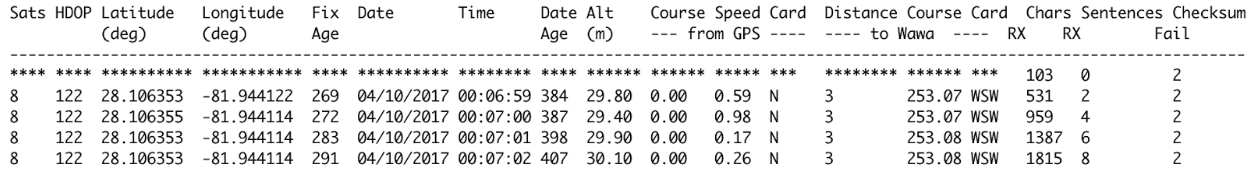
\includegraphics[width=1\textwidth]{table}
		\end{center}


In more complex navigation systems the previously mentioned code will not suffice. From this point, millions of points in the GPS coordinate system are placed in a matrix then the distance and angle between each are calculated to find the most efficient route from start to finish.

\section{Route Calculation}
\quad For a vehicle to be fully autonomous, the user would need to tell the vehicle the planned destination before leaving. The vehicle would need to then calculate the best route. The route can be calculated according to a number of factors like shortest time, shortest distance, etc. This is where graph theory comes into play. Graph theory applies linear algebra matrices to a graph of different routes that could be take in order to get from point A to point B. The graph is created where each intersection in a road would be a node, and each road between two intersections would be an edge\cite{shortRoute}.\newline

A matrix called the weighted adjacency matrix is created. This matrix is denoted M0. The values for this matrix are the “cost” for traveling between two nodes. This value can be distance, time, etc. Three new matrices are then created, which are denoted M1, M2, and M3. The first matrix, M1, has the weight values of the shortest path for the first node. M1 is essentially the same matrix as M0. M2 is the matrix with weight values for the shortest path for the second node. This process is then repeated n-1 times, and the final matrix results in the shortest weighted path between two nodes. A notable algorithm that does this is Floyd’s Algorithm \cite{shortRoute}.\newline


In a world where all cars were autonomous, graph theory could be applied to prevent traffic jams in real time, reroute cars based on real time information about traffic on the planned route, and if all autonomous cars were “connected”, could prevent the need for traffic lights at intersections. Based on research from MIT, a slot-based intersection system would drastically improve the time spent stopped at an intersection and even increase fuel efficiency. “These autonomous intersections are "slot-based," which means that they operate similarly to the way that air traffic control systems at airports coordinate landing aircraft. Air traffic controllers communicate with all incoming aircraft, and assign each one of them a specific place in the landing pattern. The individual aircraft speed up or slow down on their approach to the pattern, such that they enter it at the right time, in the right slot, and the overall pattern flows steadily.” \cite{AutonomousIntersections}
.\newline

The reason this system couldn’t be implemented right now is the lack of a way for human drivers to communicate with other drivers, and a lack of those drivers to communicate with a sort of intersection control system. The autonomous car changes that. Since all routes would be planned ahead of time, the best route could be planned using graph theory, and then the cars would have some sort of database that dictates when cars would arrive at certain intersections. This information could then be computed to let individual cars know what speeds to use while crossing an intersection in order to remove the need for stopping.



\section{Robot Vision}

Self-driving cars, such as Google’s autonomous car project, utilize a few unique methods for environmental awareness. Two main methods for self-driving cars to “see” the world around them are semantic segmentation, and a lidar-assisted parallax camera object detection system \cite{eRoad}. Systems like these, and many more like them, must have a large amount of graphics processing capability available to process images and objects around them at a high enough rate to be safe for people to use or be near\cite{Eigenfaces}.\newline 

	\begin{wrapfigure}{r}{0.4\textwidth}
		\begin{center}
			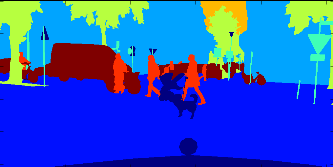
\includegraphics[width=0.4\textwidth]{5vision-2a}
		\end{center}
		\caption{RGB Sensing \cite{eRoad} }
	\end{wrapfigure}


Semantic segmentation is used by many self-driving cars as well as most technologies requiring computer vision. Most object recognition systems take an image with objects in it, break the image into a binary 2D or 3D matrix (2D for black and white, 3D for RGB values)\cite{eRoad}.\newline


\quad The objects in the matrices are recognized by software trained to look for patterns in the matrices and placing wide boxes around said images. Segmenting these matrices allows for more precise analyzation of said image. In semantic segmentation, each pixel value is assigned a classification. For a self-driving car, this allows for the car to recognize that an object isn’t part of the road and actively avoid it \cite{MatrixImages}. \newline
 
 This plays a big part in how the car stays on the road, because most roads have some combination of solid, double solid, or spaced white and yellow line segments. Not all roads are the same width and have the same turns, so this software determines what is part of the road used for motor vehicles and what might be for some other form of transportation such as bike or pedestrian lanes. This method is difficult for deciding where classified objects are relative to the car and road ahead of it, but it may be determined by pairing semantic segmentation with lidar and “parallax” cameras.\newline
 
 Being able to recognize an object in the road is very useful, but knowing how far away it is and being able to calculate if it’s moving and how to avoid it is even better. Lidar systems are laser-radar systems whose abilities include: finding distances to an object, finding basic molecular composition of weather clouds, and even mapping the entire surface of an object. The lidar system allows the car to place itself in a 3D space and know where objects around it are located. Lidar systems generally cannot cover a full 360 degree range in the time needed for a full idea of the environment for self-driving cars, so some researchers put two fish-eye cameras on their autonomous cars that constantly feed images of the car’s surroundings to its semantic segmentation software \cite{eRoad}. This allows the cameras to work together for rough distances on objects they are both looking at, as well as give the lidar some idea of what it’s pointing at so that it may move quicker. \newline
 
 Robot vision methods for self-driving cars gives them the perception needed to drive, but not quite enough. Semantic segmentation and lidar/camera systems allow the car to see, but those systems take a lot of processing power in order to be practical. To take a bit of the processing load away from these devices, some companies have even paired the lidar and the cameras with other radar systems such as sonar, but what is it that we are really processing here? The mathematics at play for object recognition is entirely matrix-based. Deep learning algorithms are useful for self-driving cars, and may be trained a variety of ways. One starts by feeding the algorithm images with various angles of one type of object (say, a car object). The algorithm will break the image down to matrix values and classify the various regions of the images depending on where the object appears in the regions. This training method goes on for thousands of images until the algorithm has an idea of what the matrix value of a “mean car” looks like, some sort of average car picture. Once it is done training, it can take a new image with a car/cars somewhere in the image. The algorithm will label where it believes the regions of the picture that could contain a car, usually by dividing the image into smaller square matrices, and then performing a few different matrix operations on the regions. In the case of convolutional neural networks, the matrices are processed against a gradient matrix to judge how accurate the data truly is that the system is receiving. \newline
 
 Training a neural network to detect objects for driving is the most important part of a usable self-driving car; without the neural network it has no ability to detect and is useless. A good example of a multi-layered neural network being trained was given by Yann LeCun, Yoshua Bengio, and Geoffrey Hinton in an article “Deep Learning” that describes the process of a multi-layered neural network \cite{deepLearning}.
	
	\begin{wrapfigure}{l}{0.5\textwidth}
		\begin{center}
			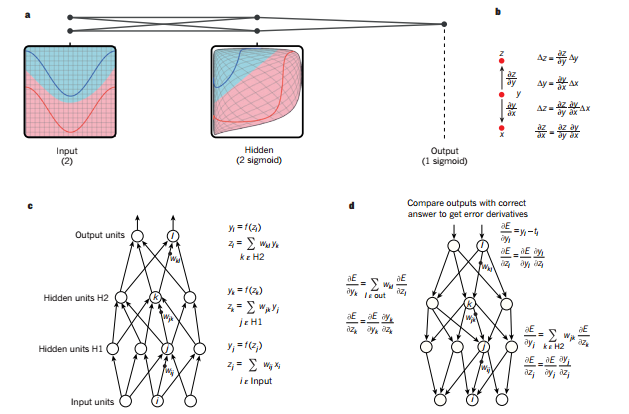
\includegraphics[width=0.5\textwidth]{recognition}
		\end{center}
		\caption{Neural Network \cite{deepLearning}}
	\end{wrapfigure}
  
  In ‘a’ we see the neural network distort the image to allow the classes of data (red/blue lines) to become linear so that it may find the changes of x on y and y on z (step ‘b’). After many iterations of chain rule, the ‘c’ step gets the unit’s z values (z is the sum of outputs of layers below), a linear function can then obtain the output of the unit. The last step ‘d’ is error checking by computing error derivatives.\newline
  
  A few different operations can be done on the region to compare it easily to the base template for the object, such as matrix: transposing to test various rotations, scalar multiplication to test various object sizes, and matrix addition for skewing the object in the image to compare with its template. When it comes to adding and scaling the matrices, the software uses changeable “weight” matrices, some matrices with numbers that will change the object in the image in such a way that the software could recognize how it relates to the template. The major problem with doing this with self-driving cars is that the self-driving car could be forced to process as much data as 1GB/s in order to function well. Perhaps over time, GPU’s may be developed specifically for self-driving cars for simplifying these matrix operations and comparisons.\newline
  

  

















\section{Conclusion}
  In conclusion, autonomous vehicles are a great example of applied linear algebra in all of its aspects. Self-driving cars heavily utilize various linear algebra techniques in its 3 main functions: GPS, graph theory calculations, and image recognition/environmental awareness. Many devices today that must do linear algebra calculations have hardware that supports the processing power needed. Self-driving cars do such a large amount of calculations that it may take some time to balance the vehicle’s processing power with its other systems to make a self-driving car as widespread a product as cell-phones and microwaves.

\newpage
\bibliographystyle{plain}
\bibliography{bib2}



\section*{Appendix}
\subsection*{Point to Point Code}
\begin{tiny}
	\lstinputlisting[language=C]{GPSProject.ino}
\end{tiny}

\subsection*{Short Route Code}
\begin{tiny}
	\lstinputlisting[language=C]{shortRoute.txt}
\end{tiny}




\end{document}
